\section{Market Dynamics and Payment}
\label{sec:payments}

\subsection{Overview}

PoAI creates a two-sided market where:
\begin{itemize}
    \item \textbf{Miners} provide AI compute and earn AI tokens
    \item \textbf{Users} pay AI tokens for AI services (inference, training, etc.)
\end{itemize}

\subsection{Payment Flow}

\begin{center}
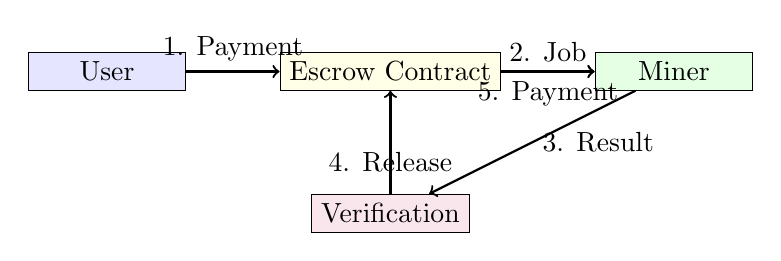
\begin{tikzpicture}[scale=0.9]
    \node[draw, rectangle, fill=blue!10, minimum width=2cm] (user) at (0,0) {User};
    \node[draw, rectangle, fill=yellow!10, minimum width=2cm] (escrow) at (4,0) {Escrow Contract};
    \node[draw, rectangle, fill=green!10, minimum width=2cm] (miner) at (8,0) {Miner};
    \node[draw, rectangle, fill=purple!10, minimum width=2cm] (verify) at (4,-2) {Verification};

    \draw[->, thick] (user) -- node[above] {1. Payment} (escrow);
    \draw[->, thick] (escrow) -- node[above] {2. Job} (miner);
    \draw[->, thick] (miner) -- node[right] {3. Result} (verify);
    \draw[->, thick] (verify) -- node[below] {4. Release} (escrow);
    \draw[->, thick] (escrow) -- node[below] {5. Payment} (miner);
\end{tikzpicture}
\end{center}

\subsection{Pricing Models}

Miners can offer multiple pricing models:

\begin{center}
\begin{tabular}{lll}
\toprule
\textbf{Model} & \textbf{Unit} & \textbf{Use Case} \\
\midrule
Per Token & AI/token & LLM inference \\
Per Inference & AI/request & Image generation \\
Per Minute & AI/minute & Real-time audio \\
Per FLOP & AI/TFLOP & Training \\
Hybrid & Mix & Custom workloads \\
\bottomrule
\end{tabular}
\end{center}

\subsection{Market-Driven Pricing}

Prices adjust based on supply and demand using \textbf{Hamiltonian market dynamics}:

\begin{definition}[Hamiltonian Market]
The market state is described by position $q$ (price) and momentum $p$ (order flow):
\begin{align}
\frac{dq}{dt} &= \frac{\partial H}{\partial p} = p \\
\frac{dp}{dt} &= -\frac{\partial H}{\partial q} - \gamma p + \xi(t)
\end{align}
where $H = \frac{p^2}{2} + V(q)$ is the Hamiltonian, $\gamma$ is damping, and $\xi(t)$ is noise.
\end{definition}

\subsubsection{Price Update Algorithm}

\begin{algorithm}
\caption{UpdateMarketPrice}
\begin{algorithmic}[1]
\Require Current price $P$, supply $S$, demand $D$, target utilization $U_{\text{target}}$
\Ensure New price $P'$
\State $U_{\text{current}} \gets D / S$ \Comment{Current utilization}
\State $\text{imbalance} \gets U_{\text{current}} - U_{\text{target}}$
\State $\text{adjustment} \gets \text{imbalance} \times \text{sensitivity}$
\State $\text{adjustment} \gets \text{adjustment} \times \text{damping}$ \Comment{Prevent oscillation}
\State $P' \gets P \times (1 + \text{adjustment})$
\State $P' \gets \max(P_{\text{min}}, \min(P_{\text{max}}, P'))$ \Comment{Bounds}
\State \Return $P'$
\end{algorithmic}
\end{algorithm}

\subsection{Escrow Contract}

Payments are held in escrow until work is verified:

\begin{lstlisting}[style=solidity]
contract ComputeEscrow {
    struct Request {
        address user;
        address miner;
        uint256 payment;
        bytes32 inputHash;
        bytes32 resultHash;
        uint256 deadline;
        RequestStatus status;
    }

    function createRequest(
        bytes32 modelId,
        bytes32 inputHash,
        uint256 maxPayment,
        uint256 deadline
    ) external returns (bytes32 requestId);

    function acceptRequest(bytes32 requestId) external;

    function submitResult(
        bytes32 requestId,
        bytes32 resultHash
    ) external;

    function verifyAndRelease(bytes32 requestId) external;

    function slashAndRefund(bytes32 requestId) external;
}
\end{lstlisting}

\subsection{Fee Structure}

\begin{center}
\begin{tabular}{lcc}
\toprule
\textbf{Fee Type} & \textbf{Rate} & \textbf{Recipient} \\
\midrule
Market Fee & 1\% & Protocol Treasury \\
Network Fee & Gas & Validators \\
Slashing & 10\% & User (refund) \\
\bottomrule
\end{tabular}
\end{center}

\subsection{Provider Registration}

Miners register as providers with stake:

\begin{lstlisting}[style=solidity]
function registerProvider(
    uint256 stake,           // Minimum 1000 AI
    bytes32 modelId,         // Supported model
    bytes32 gpuId,           // Hardware ID
    PricingModel memory pricing,
    uint256 maxConcurrent    // Max parallel jobs
) external;
\end{lstlisting}

\subsection{Slashing Conditions}

Providers are slashed (10\% of stake) for:
\begin{enumerate}
    \item \textbf{Invalid Result}: Output doesn't match input/model
    \item \textbf{Timeout}: No result by deadline
    \item \textbf{Attestation Failure}: NVTrust verification fails
\end{enumerate}

\subsection{Economic Incentives}

\begin{theorem}[Incentive Compatibility]
Under the escrow mechanism, honest behavior is a Nash equilibrium:
\begin{itemize}
    \item Miners: Providing valid compute maximizes expected profit
    \item Users: Paying for services maximizes utility
    \item Slashing cost exceeds fraud profit
\end{itemize}
\end{theorem}

\subsection{Per-Chain Fee Customization}

Each chain can set its own fee parameters:

\begin{center}
\begin{tabular}{lccc}
\toprule
\textbf{Parameter} & \textbf{Lux} & \textbf{Hanzo} & \textbf{Zoo} \\
\midrule
Base Price (AI/token) & 0.0001 & 0.0001 & 0.0001 \\
Market Fee & 1\% & 1\% & 2\% (research) \\
Min Provider Stake & 1000 AI & 1000 AI & 500 AI \\
Slashing Rate & 10\% & 10\% & 15\% \\
\bottomrule
\end{tabular}
\end{center}

This allows each chain's community to optimize for their specific use cases.
